\newcommand{\spywareTagResultsAucTable}{
    \begin{table}[H]
        \centering
        \begin{tabular}{|p{2,8cm}||p{2,8cm} p{2,8cm} p{2,8cm}|}
            \hline
            Spyware Tag & ALOHA & Joint Embedding & Proposed Model \\
            \hline
            AUC-ROC & 0.542$\pm$0.073 & \textBF{0.566$\pm$0.031} & 0.562$\pm$0.016 \\
            \hline
        \end{tabular}
        \caption{AUC-ROC (Area Under Curve) of the different models for the \textbf{Spyware Tag} prediction task. Results were aggregated over \textBF{3} training runs with different weight initializations and minibatch orderings. Best results are shown in \textbf{bold}.} \label{tab:spywareTag_auc}
    \end{table}
}

\newcommand{\spywareTagResultsAtFprTable}{
    \begin{center}
        \begin{longtable}[c]{|p{3,2cm}||p{1,8cm} p{1,8cm} p{1,8cm} p{1,8cm} p{1,8cm}|}
            \hline
            Spyware Tag & \multicolumn{5}{c|}{{FPR}} \\
            & $10^{-5}$ & $10^{-4}$ & $10^{-3}$ & $10^{-2}$ & $10^{-1}$ \\
            \hline
            \endfirsthead

            \caption*{\raggedright ...continued from previous page} \\
            \hline
            Spyware Tag & \multicolumn{5}{c|}{\textbf{FPR}} \\
            & $10^{-5}$ & $10^{-4}$ & $10^{-3}$ & $10^{-2}$ & $10^{-1}$ \\
            \hline
            \endhead

            \caption*{\raggedleft ...continued on next page} \\
            \endfoot

            \caption{Mean and standard deviation results (TPR, Accuracy, Recall, Precision and F1-Score) of the different models for the \textbf{Spyware Tag} prediction task at different \textbf{FPR}s (\textit{False Positive Rates}). Results were aggregated over \textBF{3} training runs with different weight initializations and minibatch orderings. Best results are shown in \textbf{bold}. Under \textbf{TPR} results are also presented the percentage reduction in mean detection error and in ROC curve standard deviation introduced by the \textit{Proposed Model} with respect to both \textit{ALOHA} model and \textit{Joint Embedding}.} \label{tab:spywareTag_results_at_fpr} \\
            \endlastfoot

            \multicolumn{6}{|c|}{\textbf{TPR}} \\
            \hline
            ALOHA & 0.000$\pm$0.000 & 0.000$\pm$0.000 & 0.003$\pm$0.003 & 0.016$\pm$0.005 & 0.146$\pm$0.047 \\
            Joint Embedding & \textBF{0.001$\pm$0.001} & \textBF{0.001$\pm$0.001} & \textBF{0.005$\pm$0.004} & \textBF{0.028$\pm$0.016} & \textBF{0.159$\pm$0.037} \\
            Proposed Model & 0.000$\pm$0.000 & 0.000$\pm$0.000 & 0.001$\pm$0.001 & 0.017$\pm$0.004 & 0.131$\pm$0.013 \\
            \hline
            Error Reduction wrt \newline ALOHA & 0.0\% & 0.0\% & -0.2\% & 0.1\% & -1.8\% \\
            Error Reduction wrt \newline Joint Embedding & -0.1\% & -0.1\% & -0.4\% & -1.1\% & -3.3\% \\
            \hline
            Std Reduction wrt \newline ALOHA & 0.0\% & 0.0\% & 66.7\% & 20.0\% & 72.3\% \\
            Std Reduction wrt \newline Joint Embedding & 100.0\% & 100.0\% & 75.0\% & 75.0\% & 64.9\% \\
            \hline
            \multicolumn{6}{|c|}{\textbf{Accuracy}} \\
            \hline
            ALOHA & \textBF{0.870$\pm$0.000} & \textBF{0.870$\pm$0.000} & 0.869$\pm$0.000 & 0.863$\pm$0.001 & 0.802$\pm$0.006 \\
            Joint Embedding & \textBF{0.870$\pm$0.000} & \textBF{0.870$\pm$0.000} & \textBF{0.870$\pm$0.001} & \textBF{0.865$\pm$0.002} & \textBF{0.804$\pm$0.005} \\
            Proposed Model & \textBF{0.870$\pm$0.000} & \textBF{0.870$\pm$0.000} & 0.869$\pm$0.000 & 0.863$\pm$0.001 & 0.799$\pm$0.002 \\
            \hline
            \multicolumn{6}{|c|}{\textbf{Recall}} \\
            \hline
            ALOHA & 0.000$\pm$0.000 & 0.000$\pm$0.000 & 0.003$\pm$0.003 & 0.016$\pm$0.005 & 0.146$\pm$0.047 \\
            Joint Embedding & \textBF{0.001$\pm$0.001} & \textBF{0.001$\pm$0.001} & \textBF{0.005$\pm$0.004} & \textBF{0.028$\pm$0.016} & \textBF{0.159$\pm$0.037} \\
            Proposed Model & 0.000$\pm$0.000 & 0.000$\pm$0.000 & 0.001$\pm$0.001 & 0.017$\pm$0.004 & 0.131$\pm$0.013 \\
            \hline
            \multicolumn{6}{|c|}{\textbf{Precision}} \\
            \hline
            ALOHA & \textBF{1.000$\pm$0.000} & \textBF{1.000$\pm$0.000} & 0.278$\pm$0.208 & 0.192$\pm$0.051 & 0.177$\pm$0.047 \\
            Joint Embedding & \textBF{1.000$\pm$0.000} & \textBF{1.000$\pm$0.000} & \textBF{0.367$\pm$0.262} & \textBF{0.285$\pm$0.108} & \textBF{0.191$\pm$0.035} \\
            Proposed Model & \textBF{1.000$\pm$0.000} & \textBF{1.000$\pm$0.000} & 0.111$\pm$0.157 & 0.199$\pm$0.040 & 0.163$\pm$0.014 \\
            \hline
            \multicolumn{6}{|c|}{\textbf{F1 Score}} \\
            \hline
            ALOHA & 0.000$\pm$0.000 & 0.000$\pm$0.000 & 0.006$\pm$0.005 & 0.029$\pm$0.009 & 0.160$\pm$0.048 \\
            Joint Embedding & \textBF{0.002$\pm$0.003} & \textBF{0.002$\pm$0.003} & \textBF{0.010$\pm$0.008} & \textBF{0.051$\pm$0.028} & \textBF{0.173$\pm$0.036} \\
            Proposed Model & 0.000$\pm$0.000 & 0.000$\pm$0.000 & 0.002$\pm$0.003 & 0.031$\pm$0.007 & 0.145$\pm$0.013 \\
            \hline
        \end{longtable}
    \end{center}
}

\newcommand{\spywareTagResultsSummaryTable}{
    \begin{table}[H]
        \centering
        \begin{tabular}{|p{3,2cm}||p{1,8cm} p{1,8cm} p{1,8cm} p{1,8cm} p{1,8cm}|}
            \hline
            \multicolumn{6}{|c|}{Spyware Tag (at FPR $=1\%$)} \\
            \hline
            Model & TPR & Accuracy & Precision & Recall & F1 score \\
            \hline
            ALOHA & 0.016$\pm$0.005 & 0.863$\pm$0.001 & 0.192$\pm$0.051 & 0.016$\pm$0.005 & 0.029$\pm$0.009 \\
            Joint Embedding & \textBF{0.028$\pm$0.016} & \textBF{0.865$\pm$0.002} & \textBF{0.285$\pm$0.108} & \textBF{0.028$\pm$0.016} & \textBF{0.051$\pm$0.028} \\
            Proposed Model & 0.017$\pm$0.004 & 0.863$\pm$0.001 & 0.199$\pm$0.040 & 0.017$\pm$0.004 & 0.031$\pm$0.007 \\
            \hline
        \end{tabular}
        \caption{Summary of the mean and standard deviation results of the different models for the \textbf{Spyware Tag} prediction task at \textbf{FPR} $=1\%$. Results were aggregated over \textBF{3} training runs with different weight initializations and minibatch orderings. Best results are shown in \textbf{bold}.} \label{tab:spywareTag_result_summary}
    \end{table}
}

\newcommand{\spywareTagRocAloha}{
    \begin{figure}[H]
        \vspace*{-0.5cm}
        \centering
        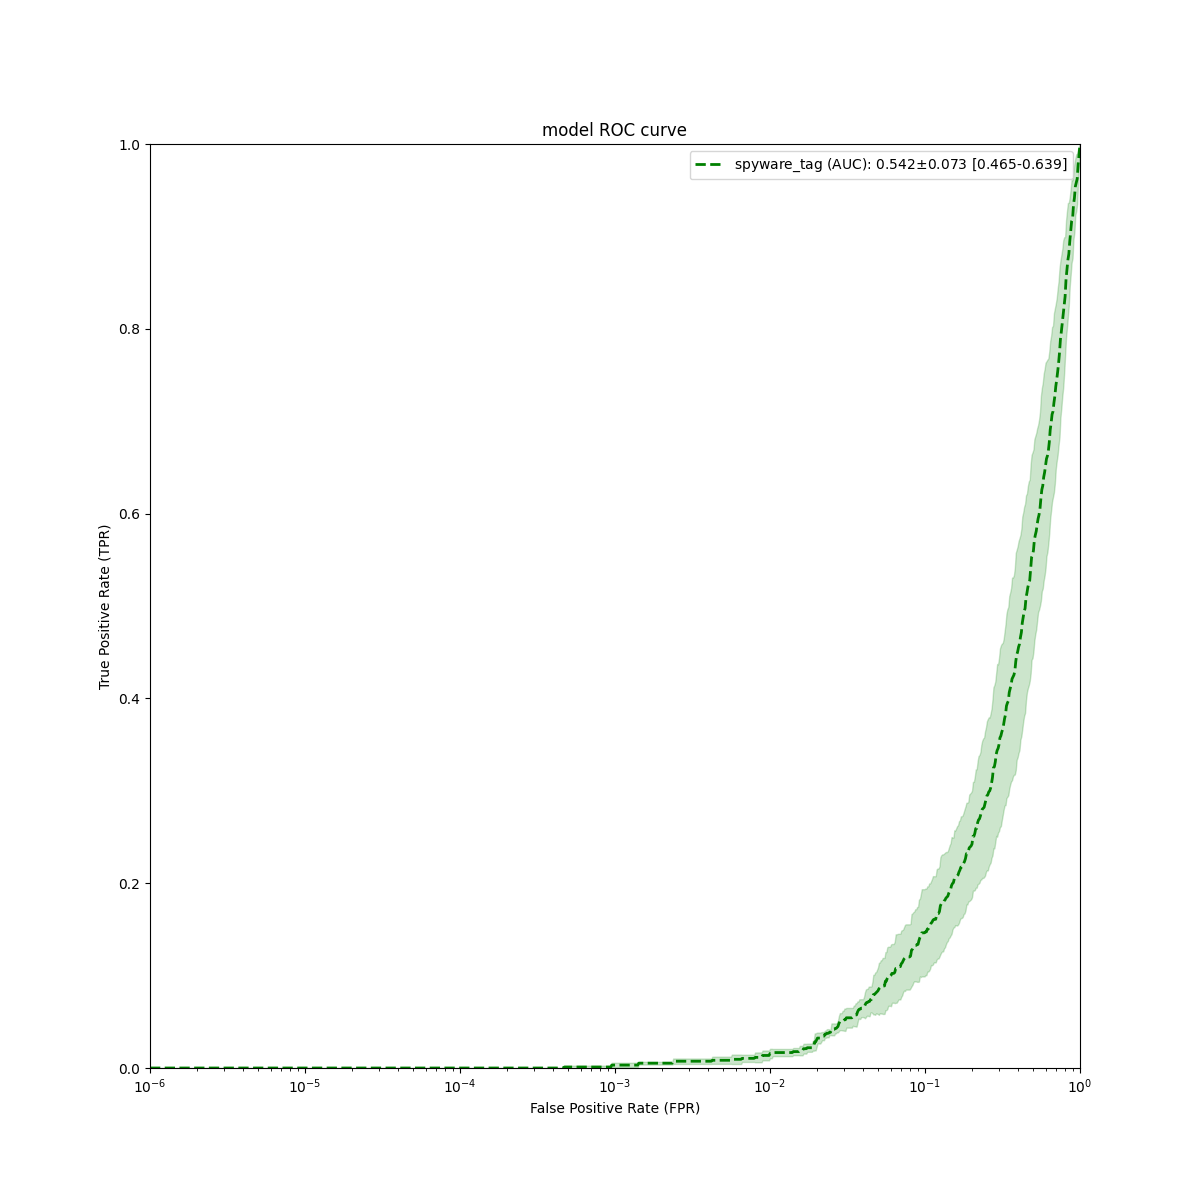
\includegraphics[width=0.6\textwidth]{./results/spyware_tag_roc_aloha.png}
        \vspace*{-0.2cm}
        \caption{ROC curve and AUC statistics of \textBF{ALOHA} model for the \textbf{Spyware Tag}. The line represents the \textit{mean} TPR at a given FPR, while the shaded region represents the \textit{standard deviation}. Statistics were computed over \textBF{3} training runs, each with random parameter initialization.}
        \label{fig:spywareTagRocAloha}
    \end{figure}
}

\newcommand{\spywareTagRocJointEmbedding}{
    \begin{figure}[H]
        \vspace*{-0.5cm}
        \centering
        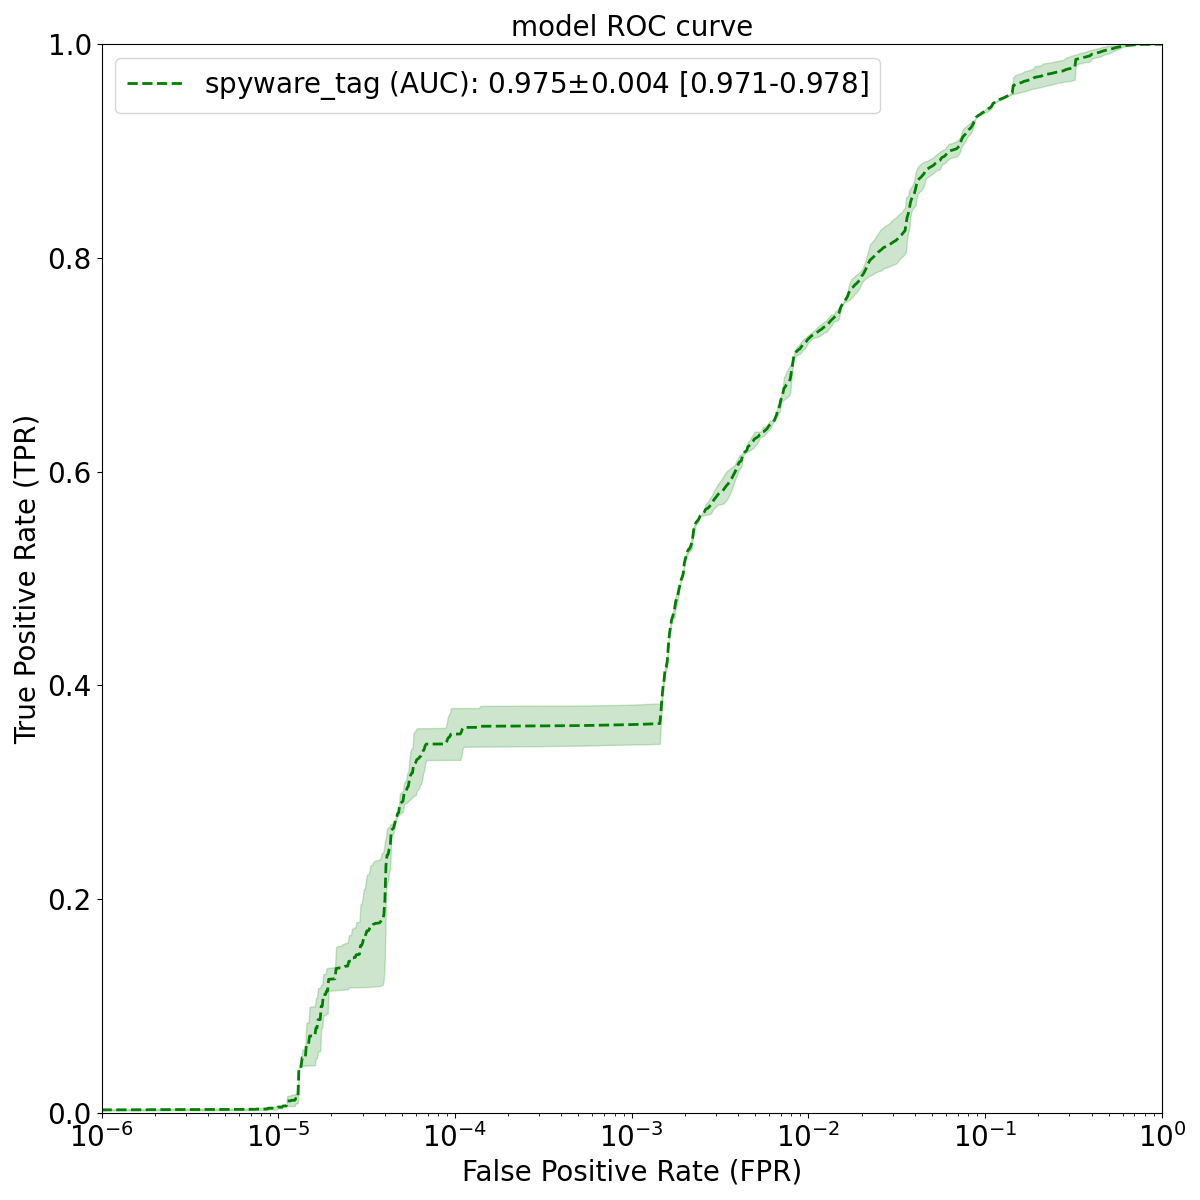
\includegraphics[width=0.6\textwidth]{./results/spyware_tag_roc_jointEmbedding.png}
        \vspace*{-0.2cm}
        \caption{ROC curve and AUC statistics of \textBF{Joint Embedding} model for the \textbf{Spyware Tag}. The line represents the \textit{mean} TPR at a given FPR, while the shaded region represents the \textit{standard deviation}. Statistics were computed over \textBF{3} training runs, each with random parameter initialization.}
        \label{fig:spywareTagRocJointEmbedding}
    \end{figure}
}

\newcommand{\spywareTagRocProposedMethod}{
    \begin{figure}[H]
        \vspace*{-0.5cm}
        \centering
        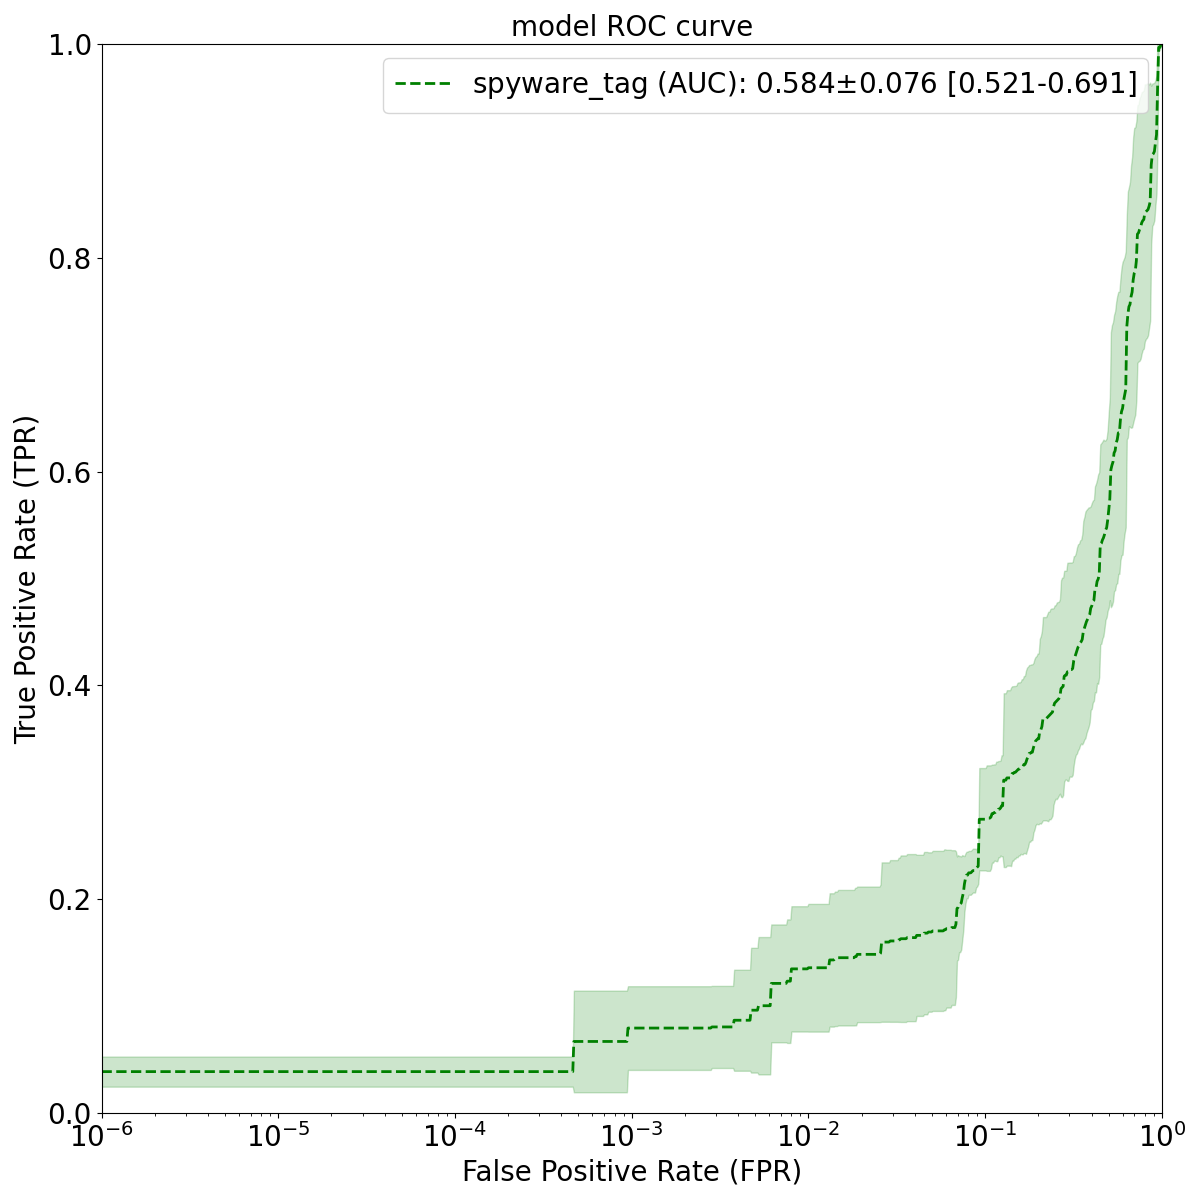
\includegraphics[width=0.6\textwidth]{./results/spyware_tag_roc_proposedModel.png}
        \vspace*{-0.2cm}
        \caption{ROC curve and AUC statistics of \textBF{Proposed Model} for the \textbf{Spyware Tag}. The line represents the \textit{mean} TPR at a given FPR, while the shaded region represents the \textit{standard deviation}. Statistics were computed over \textBF{3} training runs, each with random parameter initialization.}
        \label{fig:spywareTagRocProposedModel}
    \end{figure}
}
